
\documentclass[a4paper, 10pt]{book}
%\documentclass[10pt,technote]{IEEEtran}
%% Language and font encodings
\usepackage[english]{babel}
\usepackage[utf8x]{inputenc}
\usepackage[T1]{fontenc}
\usepackage{lmodern,babel,adjustbox,booktabs,multirow}
%%necessario per il simbolo dell'euro
\usepackage{textcomp}

%% multicolumns package
\usepackage{multicol}
%% insert figure in multicols
\usepackage{float}
%% minipage figure margin
\usepackage{caption,setspace}

%%righe nelle tabelle
%righe colorate sulle tabelle
\usepackage{xcolor}
\usepackage{color}
\usepackage{colortbl}
\definecolor{grayrow}{rgb}{0.85, 0.85, 0.85}
\definecolor{darkgrayrow}{rgb}{0.7, 0.7, 0.7}


%% Sets page size and margins
\usepackage[a4paper,top=3cm,bottom=2cm,left=2cm,right=2cm,marginparwidth=1.75cm]{geometry}

%% Useful packages
\usepackage{amsmath}
\usepackage{graphicx}
%\usepackage[colorinlistoftodos]{todonotes}
\usepackage[colorlinks=true, allcolors=blue]{hyperref}

%cartelle in cui cercare le immagini
\graphicspath{{img/}}

%% gestione degli autori
\usepackage{authblk}
\usepackage{svg}
%%\svgsetup{inkscapeexe=inkscape, inkscapearea=drawing, inkscapeversion=1}
%%\svgpath{{figures/}}
%%\newcommand{\blindcite}[1]{\textit{[reference omitted for blind review]}}
\newcommand{\quotes}[1]{``#1''}




\begin{document}
\begin{titlepage}
%
%
% ONCE YOU ARE FINISHED WITH YOUR CHANGES MODIFY "RED" WITH "BLACK" IN ALL \textcolor COMMENTS
%
%
\begin{center}
{{\Large{\textsc{Alma Mater Studiorum $\cdot$ University of  Bologna}}}} 
\rule[0.1cm]{15.8cm}{0.1mm}
\rule[0.5cm]{15.8cm}{0.6mm}
\\\vspace{3mm}
{\small{\bf School of Science \\
Department of Physics and Astronomy\\
 Degree in Physics}}
\end{center}

\vspace{17mm}

\begin{center}
%
% INSERT THE TITLE OF YOUR THESIS
%
{\LARGE{\bf EDSR-SUPER RESOLUTION DEEP LEARNING \\ \vspace{3mm}MODEL
\\
}}
\end{center}

\vspace{30mm} \par \noindent

\begin{minipage}[t]{0.47\textwidth}

{\large{\bf Supervisor: \vspace{2mm}\\
Prof. Daniel Remondini\\\\

\bf Co-supervisor:
\vspace{2mm}
\\
Dr. Nico Curti\\\\}}
\end{minipage}
%
\hfill
%
\begin{minipage}[t]{0.47\textwidth}\raggedleft \textcolor{black}{
{\large{\bf Submitted by:
\vspace{2mm}\\
Andrea Corvina}}}
\end{minipage}

\vspace{40mm}

\begin{center}

Academic Year 2021/2022
\end{center}

\end{titlepage}





%%\newcommand{\blindcite}[1]{\textit{[reference omitted for blind review]}}


\date{}

\newpage

\vspace*{125px}
\LARGE\textit{Abstract}
\normalsize
\vspace{2mm}



\newpage
\normalsize 


\tableofcontents

\newpage

\chapter{Introduction}
The computer-assisted analysis for enhancing images have been longstanding issues in different field:
\begin{enumerate} 

\item surveillance: to detect, identify, and perform facial recognition on low-resolution images obtained from security cameras.
\item medical: capturing high-resolution MRI images can be tricky when it comes to scan time, spatial coverage, and signal-to-noise ratio (SNR). Super resolution helps resolve this by generating high-resolution MRI from otherwise low-resolution MRI images.
\item media: in order to reduce server costs, as media can be sent at a lower resolution and up-scaled on the fly.
\end{enumerate}
In order to obtain an high resolution image it is necessary to enlarge the dimension of a  low resolution image, i.e upsample the image. There are different methods for image upsampling, some of them are simple interpolation methods and other are deep learning methods.
The former comprises bicubic interpolation,the latter comprises super resolution methods like WDSR and EDSR.
In this work I will study the the performances of EDSR -Deep
Learning Single Image Super-Resolution model on different type of images.
In particular I will compare super resolved images with bicubic upsampled images.
To evaluate numerically the quality of the image before and after the super resolution and to compare upsampled images  with two different methods I will use SSIM and PSNR.
In this work I will apply upsampling methods on different kind of images: medical Grey-scale images, and RGB images.

\section{ Digital Image}
Digital images are made of elements called pixels.  Typically, pixels are organized in an ordered rectangular array.  The size of an image is determined by the dimensions of this pixel array.  The image width is the number of columns, and the image height is the number of rows in the array.  Thus the pixel array is a matrix of M columns x N rows.  To refer to a specific pixel within the image matrix, we define its coordinate at x and y.  The coordinate system of image matrices defines x as increasing from left to right and y as increasing from top to bottom.  Compared to normal mathematic convention, the origin is in the top left corner and the y coordinate is flipped. Originally, digital images were defined in terms of the electron beam scanning pattern of televisions.  The beam scanned from left to right and top to bottom.  Other than this historical reason, there is no purpose served by this inversion of the y coordinate.
\subsection{Grey-scale Image}
In digital photography, computer-generated imagery, and colorimetry, a grey-scale image is one in which the value of each pixel is a single sample representing only an amount of light; that is, it carries only intensity information. 
Grey-scale images are distinct from one-bit bi-tonal black-and-white images, which, in the context of computer imaging, are images with only two colors: black and white (also called bilevel or binary images). Grayscale images have many shades of gray in between.
Each of the pixels that represents an image stored inside a computer has a pixel value which describes how bright that pixel is, and/or what color it should be. In the simplest case of binary images, the pixel value is a 1-bit number indicating either foreground or background. For a Grey-scale images, the pixel value is a single number that represents the brightness of the pixel. The most common pixel format is the byte image, where this number is stored as an 8-bit integer giving a range of possible values from 0 to 255. Typically zero is taken to be black, and 255 is taken to be white. Values in between make up the different shades of gray.
\subsection{RGB  Images}
RGB (red, green, and blue) refers to a system for representing the colors to be used on a computer display. An RGB image is a 3- Dimensional image. There is one channel for each color. Red, green, and blue can be combined in various proportions to obtain any color in the visible spectrum. Levels of R, G, and B can reach range from 0 to 100 percent of full intensity. Each level is represented by the range of decimal numbers from 0 to 255 (256 levels for each color). The total number of available colors is 256 x 256 x 256, or 16,777,216 possible colors.


\subsection{PSNR}
Peak signal-to-noise ratio (PSNR) is a term for the ratio between the maximum possible power of a signal and the power of corrupting noise that affects the fidelity of its representation. 
Because many signals have a very wide dynamic range, PSNR is usually expressed as a logarithmic quantity using the decibel scale.
PSNR is commonly used to quantify reconstruction quality for images and video subject to lossy compression.
PSNR is most easily defined via the mean squared error (MSE). Given a noise-free m×n monochrome image I and its noisy approximation K, MSE is defined as
\begin{equation}\label{eqn:MSE}
{\displaystyle {\mathit {MSE}}={\frac {1}{m\,n}}\sum _{i=0}^{m-1}\sum _{j=0}^{n-1}[I(i,j)-K(i,j)]^{2}.}{\displaystyle {\mathit {MSE}}={\frac {1}{m\,n}}\sum _{i=0}^{m-1}\sum _{j=0}^{n-1}[I(i,j)-K(i,j)]^{2}.}
\end{equation}

The PSNR (in dB) is defined as
\begin{equation}\label{eqn:PSNR}
{\displaystyle {\begin{aligned}{\mathit {PSNR}}&=10\cdot \log _{10}\left({\frac {{\mathit {MAX}}_{I}^{2}}{\mathit {MSE}}}\right)\\&=20\cdot \log _{10}\left({\frac {{\mathit {MAX}}_{I}}{\sqrt {\mathit {MSE}}}}\right)\\&=20\cdot \log _{10}({\mathit {MAX}}_{I})-10\cdot \log _{10}({\mathit {MSE}}).\end{aligned}}}
\end{equation}
\\
Here, $MAX_I$ is the maximum possible pixel value of the image. When the pixels are represented using 8 bits per sample, this is 255. More generally, when samples are represented using linear PCM with B bits per sample, $MAX_I$ is 2B − 1.
\\
For color images with three RGB values per pixel, the definition of PSNR is the same except that the MSE is the sum over all squared value differences (now for each color, i.e. three times as many differences as in a monochrome image) divided by image size and by three. Alternately, for color images the image is converted to a different color space and PSNR is reported against each channel of that color space.

\subsection{SSIM}
SSIM is a perception-based model that considers image degradation as perceived change in structural information, while also incorporating important perceptual phenomena, 
including both luminance masking and contrast masking terms. The difference with other techniques such as MSE or PSNR is that these approaches estimate absolute errors.
 Structural information is the idea that the pixels have strong inter-dependencies especially when they are spatially close. 
 These dependencies carry important information about the structure of the objects in the visual scene. 
 Luminance masking is a phenomenon whereby image distortions (in this context) tend to be less visible in bright regions, while contrast masking is a phenomenon whereby distortions become less visible where there is significant activity or "texture" in the image.
 \begin{equation}
    \label{eqn:SSIM}
SSIM(I,K) =1/N \sum\limits_{i=1}^N SSIM_{i}x{i},y{i})
\end{equation}
where N is the number of the windows in the image.
 The SSIM index is calculated on various windows of an image. The measure between two windows ${\displaystyle x}$ and ${\displaystyle y}$ of common size ${\displaystyle N\times N}$  is:

 \begin{equation}\label{eqn:SSIM_DOUBLE}
 {\displaystyle {\hbox{SSIM}}(x,y)={\frac {(2\mu _{x}\mu _{y}+c_{1})(2\sigma _{xy}+c_{2})}{(\mu _{x}^{2}+\mu _{y}^{2}+c_{1})(\sigma _{x}^{2}+\sigma _{y}^{2}+c_{2})}}}{\displaystyle {\hbox{SSIM}}(x,y)={\frac {(2\mu _{x}\mu _{y}+c_{1})(2\sigma _{xy}+c_{2})}{(\mu _{x}^{2}+\mu _{y}^{2}+c_{1})(\sigma _{x}^{2}+\sigma _{y}^{2}+c_{2})}}}
 \end{equation}

with:

$$ {\displaystyle \mu _{x}}{\text{ the average of }} {\displaystyle x};$$
$$ {\displaystyle \mu _{y}} {\text{ the average of }} {\displaystyle y};$$
 $${\displaystyle \sigma _{x}^{2}}{\text{ the variance of }} {\displaystyle x};$$
 $${\displaystyle \sigma _{y}^{2}}{\text{ the variance of  }}{\displaystyle y};$$
 $${\displaystyle \sigma _{xy}}{\text{ the covariance of }} {\displaystyle x} {\text{ and }} {\displaystyle y};$$
$$ {\displaystyle c_{1}=(k_{1}L)^{2}},$$
$${\displaystyle c_{2}=(k_{2}L)^{2}}$$
 two variables to stabilize the division with weak denominator;
$$ {\displaystyle L}$$ the dynamic range of the pixel-values (typically this is ${\displaystyle 2^{\#bits\ per\ pixel}-1}{\displaystyle 2^{\#bits\ per\ pixel}-1});$
 $${\displaystyle k_{1}=0.01} {\text{ and }} {\displaystyle k_{2}=0.03}$$ {\text{  by default.}}

\subsection{bicubic interpolation}

The Bicubic interpolation is a common algorithm used in image analysis either to downsample or upsample an image. This operation is also called re-scaling and its purpose is to interpolate the pixel values after a resize of the image, respectively after shrinking or expanding it, e.g as a consequence of zooming. The name comes from the highest order of complexity of the operation used in the algorithm, which is a cubic function. Given
a pixel, the interpolation function evaluates the 4 pixel around it by applying a filter defined as:
\begin{equation}
    \label{eqn:bicubic}
{\displaystyle W(x)={\tfrac {1}{6}}{\begin{cases}(12-9B-6C)|x|^{3}+(-18+12B+6C)|x|^{2}+(6-2B)&{\text{if }}$$|x|< 1$$,\\(-B-6C)|x|^{3}+(6B+30C)|x|^{2}+(12B-48C)|x|+(8B+24C) &{\text{if}}1\leq|x|<2,\\0&{\text{otherwise}},\end{cases}}}
\end{equation}
\\
where x identifies each pixel below the filter. Common values used for the filter parameters are B = 0 and C = 0:75 (used by OpenCV library) or B = 0 and C = 0:5 used by Matlab and Photoshop. The scale factor of the down/up sampling can assume different values according to the user needs; for this work, I used an upsampling factor of x2 and the algorithm is from the Python version of the library OpenCV [6]. The
main aims of SR algorithms are to provide a better alternative to standard upsampling and obtain a better quality image both from a qualitative (visual perception) and a quantitative point of view.


\chapter{Neural Network}
\section{What is a Neural Network?}
Neural networks are function approximator used in data analysis.
They are an essential instrument for  machine learning  and deep learning reaserch. They descend  from the works on learning and neural plasticity of Donald Hebb: an attempt to describe the animals' brain.
He attempted to explain the  change of strenght in  neural relations as a consequence of stimulations.
From the so called Hebbian theory , arose \quotes {the perceptron}(the first computational model by Frank Rosenblatt),Neural Networks and the modern Deep Learning.
\\
From a theoretical point of view  Neural Networks are defined by a sequences of non linear  multi-parametric  functions, to create an interconnected structure of simple procedural units.
The parameters are tuned during the \quotes{training phase}by minimizing the error function ,i.e loss, starting from random values.
\\
Machine learning problems are optimization problems where through iterative operations, we can approximate the correct result.
Solutions are not in an analytic form and the iterative methods are generally some kind of gradient descent.
\\
The model has three different methods of learning:
\begin{enumerate}
  

\item  supervised learning, during the training session, with the user' supervision, a set of data are provided to the model.
The model's  outcome is compared with the right output, therefore the model can variate  his own parameters to produce the desire result.
Some problems tied to supervised algorithms are classification, regression, object
detection, segmentation and super-resolution.
\item unsupervised learning, in this case there is not a correct set of data that can be used as comparison.The training procedure must be tailored around the problem under study. Some examples of unsupervised algorithms are clustering, auto-encoders,
anomaly detection.
\item  reinforcement learning, the model interacts with a dynamic environment and tries to reach a goal (e.g. winning in a competitive game). For each iteration of the training process we assign a reward or a punishment, relatively to the progress in reaching the objective.
   
\end{enumerate}
This work will focus on models trained using labeled samples, therefore in a supervised environment.

\section{Simple Perceptron}

The simple perceptron (or single neuron) is the fundamental unit of every Neural Network.
It is a simple  model for a biological neuron. From \quotes{Rosenblatt  model}
a neuron is a computational unit with input, synaptic weights and activation  functions. The perceptron receives N inputs values and produces an output that is a linear combination of them plus a bias.


\begin{equation}\label{eqn:perceptron}
     y = \sigma ( \sum\limits_{i=1}^N w_i x_i +w_0) 
\end{equation} 
\\
where $\sigma$ is the activation function,$
w_i$ are the synaptic weights and $x_i$ the inputs;
$w_0$ is the coefficient that identifies the bias of the linear combination. It is a parameter that has to be tuned by the optimizer algorithm (learning phase). Originally, the activation function was the Heaviside step function whose value is zero for negative arguments and one for non-negative arguments:

        \begin{equation}
            \label{eqn:Heaviside}
         {\displaystyle H(x) := \begin{cases}0 &{\text{if }}$$x< 0$$,\\1 &{\text{if }} x\ge 0 \end{cases}}
            \end{equation} 
\\        
therefore the perceptron became a linear discriminator able to learn an hyperplane which linearly separates two set of data.
The wights$ w_i$ are tuned during the training phase following the chosen updating rule. The standard updating rule, usually:

\begin{equation}
    \label{eqn:standard_updating_rule}
w_i (\tau +1) = w_i (\tau) + \eta(t - y)x 
\end{equation}
\\
Where $\eta$ is the learning rate,or gain factor that controls how fast we train and t is the true output.
\\
If the input instance is correctly classified , the error(t-y) is zero.
Otherwise, the hyperplane is moved towords the missclassified example.
Repeating this process will lead to a convergence only if the two classes are linearly separable. This model presents numerous limits. The output function is a simple linear combination of the input with a vector of weights and so only linearly separable problems can be learned  by the Perceptron. Moreover we can manage only two classes since an hyper-plane divide the space in only two half-spaces.

\section{Fully connected Network}

The direct generalization of a simple perceptron is the fully connected Artificial Neural Network. In this model, multiple perceptron units, following the computation formula (\ref{eqn:perceptron}), are joined together in a more complex  network. 
They form a multilayer structure in wich the output of a neuron feeds-forward the input of the next one (multy-layer perceptron). 
Every neuron is  also connected to all the other in order to create the fully connected Neural Network.
A typical representation of this type of network is shown in figure \ref{fgr:neural_net}:

\begin{figure}[htp]
    \centering
    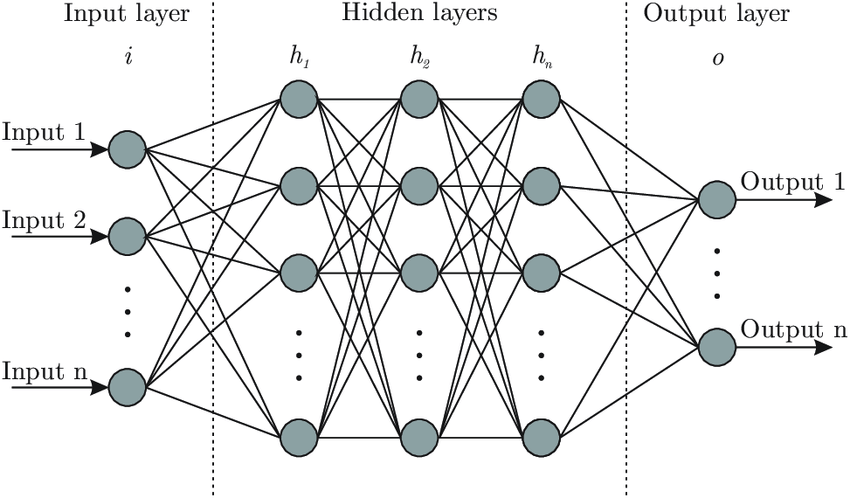
\includegraphics[width=12cm]{neural_net.png}
    \caption{fully connected network}
    \label{fgr:neural_net}
\end{figure}


The mathematical generalization from the perceptron is simple, indeed given the i-th layer its output vector $y_i$ reads:

\begin{equation}
    \label{eqn:fully_conncect}
{y_i = \sigma (W_i y_{i-1}+ b_i) }  
\end{equation}
\\
where $ W_i$ is the weights matrix of layer i and $b_i$ is the i-th bias vector, equivalent to $w_0$ in the perceptron case. The output of the i-th layer becomes the input of the next one until the output layer yields the network's answer.
As before, $\sigma$ is the activation function which can be different for every node, but it usually differs only from layer to layer. How to chose the best activation function is yet to be understood, and most works rely on experimental results.
\\
As in the single perceptron, in a supervised environment the output of a multi-layer perceptron is compared to the desired one by a cost function:

\begin{equation}
    \label{eqn:cost_function}
C(W) = \frac{1}{N} \sum \limits_{j=1}^N (y_j - t_j)^2
\end{equation}
where N is the dimensionality of the output space. C is considered as a function of the model's weights only since input data and truth labels t are fixed. The most simple updating rule is the gradient descent:

\begin{equation}
    \label{eqn:updat_g_discent}
w  \leftarrow   w-\eta \nabla_w C
\end{equation}
The core idea is to modify the parameters by a small step in the direction that minimizes the error function. The length of the step is given by the learning rate $$\eta  $$ which is a hyper-parameter chosen by the user, while the direction of the step is given by $$ \nabla_w C $$ which point towards the steepest descent of the function landscape.
More efficient updating rules exist but they follow the gradient descent updating rule.

\section{Error Backprpagation}
Our goal in this section is to find an efficient technique for evaluating the gradient
of an error function E(w) for a feed-forward neural network. We shall see that this can be achieved using a local message passing scheme in which information is sent alternately forwards and backwards through the network and is known as error backpropagation.
we first introduce the error energy.
\begin{equation}
    \label{eqn:Error Energy}
E(W)= \sum\limits_{N=1}^N E_n(W).
\end{equation}
\\
We have to chose the right vector W due to minimize  the error function E(w).
It is useful to have a geometrical picture of the error function, 
which we can view as a surface sitting over weight space as shown in
Figure \ref{fgr:gradient}.
\begin{figure}[H]
    \centering
    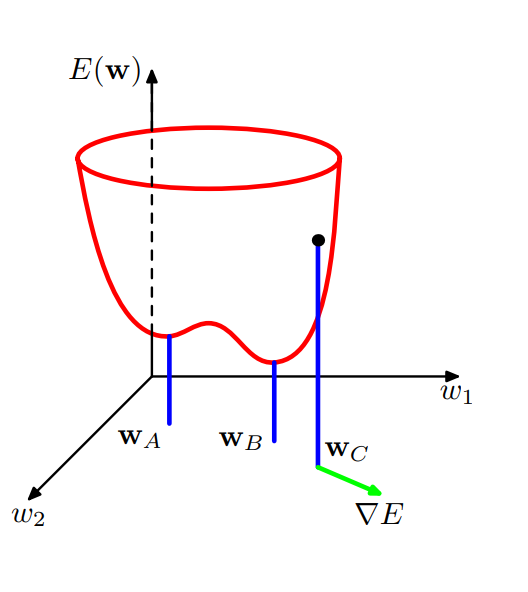
\includegraphics[scale=1]{gradient_sr_1.png}
    \caption{Geometrical view of the error function E(w) as
a surface sitting over weight space. Point $w_A$ is
a local minimum and $w_B$ is the global minimum.
At any point $w_C$ , the local gradient of the error
surface is given by the vector $\nabla $E.}
\label{fgr:gradient}
\end{figure}
Because the error E(w) is a smooth continuous function of w, its smallest value will occur at a
point in weight space such that the gradient of the error function vanishes, so that
\begin{equation}
    \label{eqn:gradient E}
\nabla  E(W) = 0
\end{equation}
\\
Our goal is to find a vector such that E(w) takes its smallest value. 
However, the error function typically has a highly nonlinear dependence on the weights and bias parameters, and so there will be many points in weight space at which the gradient vanishes .
For a successful application of neural networks, it may not be necessary to find the global minimum (and in general it will not be known whether the global minimum has been found) but it may be necessary to compare several local minima in order to find a sufficiently good solution.
\\
Many algorithms make use of gradient information and therefore require that, after each update, the value of $\nabla$E(w) is evaluated at the new weight vector $w ( \tau +1 ) $. 
\\
Most training algorithms involve an iterative procedure for minimization of an error function, with adjustments to the weights being made in a sequence of steps. At each such step, we can distinguish between two distinct stages. In the first stage, the derivatives of the error function with respect to the weights must be evaluated. As we shall see, the important contribution of the backpropagation technique is in providing a computationally efficient method for evaluating such derivatives. Because it is at this stage that errors are propagated backwards through the network, we shall use the term backpropagation specifically to describe the evaluation of derivatives.
In the second stage, the derivatives are then used to compute the adjustments to be made to the weights
\\
The error  backpropagation process can be resumed in 4 steps:
\begin{enumerate}

\item	We first apply an input vector $x_n$ to the network and forward propagate through the network
 using for each units a weighted sum of its inputs of the form:
\begin{equation}
    \label{eqn:sum inputs}
 a_j = \sum\limits_{i} w_(ji)z_i   
\end{equation}
with $w_{ji}$ the weights associated with that connection.
The sum in \ref{eqn:sum inputs} is
transformed by a nonlinear activation function $h(\cdot)$  to give the activation $z_j$ of unit j
in the form:
\begin{equation}
    \label{eqn:activated out}
z_j = h(a_j).                       
\end{equation}
For each pattern in the training set, we shall suppose that we have supplied the corresponding input vector to the network and calculated the activation of all of the hidden and output units 
in the network by successive application of \ref{eqn:sum inputs} and \ref{eqn:activated out}. This process is often called forward
propagation because it can be regarded as a forward flow of information through the network.
	
\item	Than   to Evaluate the $\delta_k$ for all the output units we have:
 \begin{equation}
     \label{eqn:delta}
 \delta_k = y_k − t_k  
 \end{equation}
\item	We backpropagate the $\delta $ backwards from units higher up in the network due to obtain the $\delta$ of a particular hidden layer using the formula :
\begin{equation}
    \label{eqn:delta hidden layer}
    \delta_j = h'(a_j)\sum\limits_{k} w_(ki)\delta_k  
  \end{equation}
    That is obtained making use of the chain rule for partial derivatives as follow:
    \begin{equation}
        \label{eqn:chain rule}
   \delta_j =\frac{\partial E_n}{\partial a_j} = \sum\limits_{k}\frac{\partial E_n}{\partial a_k} \frac{\partial a_k}{\partial a_j}
  \end{equation}
    where the sum runs over all units k to which unit j sends connections. Note that the units labelled k could include other hidden units and/or output units. 
    In writing down (\ref{eqn:chain rule}), we are making use of the fact that variations in $a_j$ give rise to variations in the error function only through variations in the variables $a_k$.

\item	The required derivatives are evaluated using:
   \begin{equation}
       \label{eqn:deriv_costfunc_w}
   \frac{\partial E_n}{\partial w_{ji}} = \delta_j z_i
   \end{equation}  
   where $\delta_j$ givn by equation \ref{eqn:chain rule} and:
   \begin{equation}
       \label{eqn:z_i}
     z_i= \frac{\partial a_j}{\partial w_{ji}  }
\end{equation}
\end{enumerate}

\newpage
\section{Super Resolution}

The Super Resolution (SR) is a slight novel technique based on Neural Network models which aims to improve the spatial resolution of a given image.
\\
Super-resolution  (SR) is a class of techniques that enhance (increase) the resolution of an imaging system. Thus converting a given low resolution (LR) image to a corresponding high resolution (HR) one, with better visual quality and refined details.
Image super-resolution is also called by other names like image scaling, interpolation, upsampling and zooming.
HI provides an improved reconstructed details of the scene and object of the image.
\\
We can distinguish from single image super resolution and multiple image super resolution. In this work we will conceatre on single image super reoslution SISR
\\
Fields of application for super resolution:
object detection in scenes, face recognition in surveillance videos, medical imaging, improving interpretation of images in remote sensing, astronomical images, and forensics.
\\
SR is  still a challenging problem and an import research topic for two main reasons:
\begin{enumerate}
\item it is a ill-posed inverse problem,i.e there exist multiple solution for the same low resolution image, the domain has to be restricted 
\item Its complexity depends on the up-scale factor used, i.e with increasing up-scale factors, the problem complexity increases.
\end{enumerate}
Super resolution can broadly divided in two groups:
traditional  and deep learning methods\cite{https://doi.org/10.48550/arxiv.1904.07523}.

\subsection{Traditional method}
We can define the degradation model as:
\begin{equation}
    \label{first SR}
    y = {x \otimes k } + n 
\end{equation}
with y is the LR image, X  is the HR image, K is the blurring down-sampling kernel.
\\
In image super resolution, the aim is to minimize the data fidelity term associated with the model, as
\begin{equation}
    \label{fidelty equation}
    J(\hat{x} , \theta _\xi , k ) = ||{x \times k - y}|| +  \alpha \Psi(X\Theta_\xi) 
\end{equation}
\subsection{Deep learning methods} 
There are different SISR model. The earliest and simplest  models were based on linear networks.
They have a simple structure consisting of only
a single path for signal flow without any skip connections
or multiple-branches.
Linear networks differ in the way the up-sampling operation is performed i.e., early upsampling or late upsampling.
\subsubsection{ Early upsampling}
The early upsampling designs are linear networks that first
upsample the LR input to match with desired HR output size and then learn hierarchical feature representations to
generate the output. 
A common upsampling operation used for this purpose is Bicubic interpolation, which is a computationally expensive operation. 
\\ 
An example of linear early method is SRCNN. super resoluition convolutional neural network.
It only consists of convolutional layers where each layer (except the last one) is followed by rectified linear unit (ReLU) non-linearity. There are a total of three convolutional and two ReLU layers, stacked together
linearly. The SRCNN is an end-to-end trainable network and minimizes the difference between the output reconstructed high-resolution images and the ground truth high-resolution images using Mean Squared Error (MSE) loss function.
\subsubsection{Late upsampling}
Late upsampling model instead of upsample the image at the beginning (computatinally expansive), practice a post-upsampling, i.e they perform the learning on the low-resolution inputs and then upsample the features near the output of the network.
This strategy results in efficient approaches with low memory footprint. 
\subsection{Residual Neural Network}
In contrast to linear networks, residual learning uses skip
connections in the network design to avoid gradients vanishing and makes it feasible to design very deep networks.
In this approach, algorithms learn residue i.e. the high frequencies between the input and ground-truth. 
An example of RSNN is EDSR:  The Enhanced Deep Super-Resolution (EDSR) modifies the ResNet architecture  proposed originally for image classification to work with the SR task. Specifically, they demonstrated substantial improvements by removing Batch Normalization layers (from each residual block) and ReLU activation (outside residual blocks).
The creator of this Network extended this single scale SR to a multiple scale SR, the MDSR.
EDSR and MDSR achieve better performance, in terms of quantitative measures ( e.g., PSNR), compared to older architectures such as SR-CNN and other ResNet based closely related architectures.
\\
\\
\\

\section{Algorithms}
As described above, a neural network can be considered as a composition of function:
 for this reason every Deep Learning framework (e.g. Keras/Tensor ow, Pytorch, Darknet)
 implement each function as an independent object called Layer.
 By stacking different kind of layers one after another, it is possible to build complex
 models with tens of millions of parameters. For the purposes of this work, I'm going
 to describe layers used in super resolution.

\subsection{Layers}
In deep learning, a convolutional neural network (CNN, or ConvNet) is a class of artificial neural network (ANN), most commonly applied to analyze visual imagery.[1]
 CNNs are also known as Shift Invariant or Space Invariant Artificial Neural Networks (SIANN), based on the shared-weight architecture of the convolution kernels  or filters that slide along input features and provide translation-equivariant responses known as feature maps.[2][3]
 Counter-intuitively, most convolutional neural networks are not invariant to translation, due to the downsampling operation they apply to the input.[4] 
 They have applications in image and video recognition, recommender systems,[5] image classification, image segmentation, medical image analysis, natural language processing,[6] 
 brain–computer interfaces,[7] and financial time series.[8]

\subsubsection{Convolutional layer}
Convolutional neural network (CNN)  are specialized kind of neural network for processing data that has a know like grid topology, like images. The name convolutional indicates that they employ a particular mathematical operation called convolution.
In its most general form, convolution is an operation on two functions of a real-valued argument.
\begin{equation}
    \label{eqn:conv_layer}
(f\star g) (t) = \int_{-\infty}^{+\infty} f(\tau)g(t-\tau) d\tau \\
\end{equation}
 In convolutional network terminology, the first argument (the first function) to the convolution is often referred to as the input, and the second argument (the second function) as the kernel. The output is referred to as the feature map.
 In machine learning applications, the input is usually a multidimensional array of data, and the kernel is usually a multidimensional array of parameters that are adapted by the learning algorithm.
 We often use convolutions over more than one axis at a time. For example, if we use a two-dimensional image I as our input, we probably also want to use a two-dimensional kernel K:
 \begin{equation}
     \label{eqn:2_dimension_conv}
  S(i, j) = (I ∗ K)(i, j) =\sum m \sum n I(m, n)K(i − m, j − n).
 \end{equation}
Where s(i,j ) is the pixel value of the output image and N,M are the kernel dimension.
CNN are specifically designed to process pixel data and are used in image recognition and processing.
Practically speaking, a convolution is performed by sliding a kernel of dimension $ N X M $ over the image, every kernel position correspond to a output pixel, the value of that is calculated by multiplying together the kernel value and the underlying pixel value for each cell of the kernel and summing all the results, as shown in figure \ref{fig:conv_layer}:

\begin{figure}[htp]
    \centering
    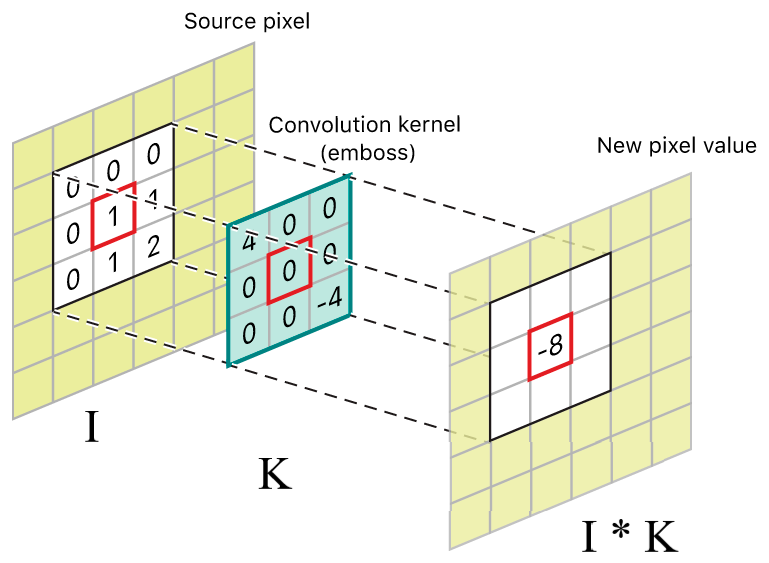
\includegraphics[width=15cm]{conv.png}
    \caption{Visual example of convolution of an image I 6x6 with a 3x3 kernel K}
    \label{fig:conv_layer}
\end{figure}
A feature map is so created and it’s is passed to the next layer
CNN can be interpreted like a filter. By choosing the right kernel (filter) it is possible to highlight different features. 
For this reason the convolution operation is commonly used in image analysis: some of the most common applications are denoising, edge detection and edge enhancement.
\\
The convolutional layer (CL) object is the most used layer in DL image analysis, therefore its implementation must be as efficient as possible. Its purpose is to perform multiple (sometimes thousands) convolution over the input to extract different high-level features, which are compositions of many low-level attributes of the image (e.g edges,simple shapes). 
This is similar to the response of a neuron in the visual cortex to a specific stimulus: each convolutional neuron processes data only for its receptive field and shares parameters with all the neuron spatially close.
As more CL are stacked the receptive field of a single neuron grows and with that the complexity of the feature it can extract.
The local nature of the receptive field make the model independent from translation.
There’s not determined parameters, the weight are tuned during the training phase. A CL is defined by the following parameters: 
\begin{enumerate}

\item	Kernel size, it is the size of the sliding filters. The depth of the filter(number of channels) is the same of the input image. Other dimensions (width and height) don’t  have  any limitation but usually implementations require squared kernels
\item	Strides, tehy define the sliding of the filter over input image. With a low stride there is an overlapping. With an high stride the overlap can vanish and the output dimension can decrease.
\item	Number of filters (depth), it is the number of filters that are applied on the input.
\item	Padding, it is the dimension of an artificial enlargement of the input image, necessary for the application of the filters on borders.
\end{enumerate}

It is possible to compute the number of weights and bias needed for the initialization of the CL.
We start from an image of dimension (H,W,C) slided by n different 3-D filters of size$(k_x,k_y) $with stride $(s_x,s_y)$ and padding p,then:
\begin{equation}
    \label{weights}
 weights = n \times k_x \times k_y \times C
\end{equation}
\begin{equation}
    \label{bias}
 bias = n
\end{equation}
The number of weights don’t depend on the dimension of the input, but only on his depth. This means that a CL can work on images of every size, as they have the correct depth.
The output dimensions are ($out_H$; $out_W$;n) where:

\begin{equation}
    \label{out_h}
out_H = \frac{H-K_x +p}{s_x} +1\end{equation}
\begin{equation}
    \label{out_W}
out_W = \frac{W-K_y +p}{s_y} +1\end{equation}


Even if the operation can be implemented as described above in equation \ref{eqn:2_dimension_conv}, this is never the case, in fact a discrete convolution can be viewed as a single matrix multiplication.
The first matrix has as rows each filters of the CL, while the second matrix has as columns every windows of the image traversed by the kernels,
as shown in figure \ref{fig: convolutional layer _2}.
\begin{figure}[htp]
    \centering
    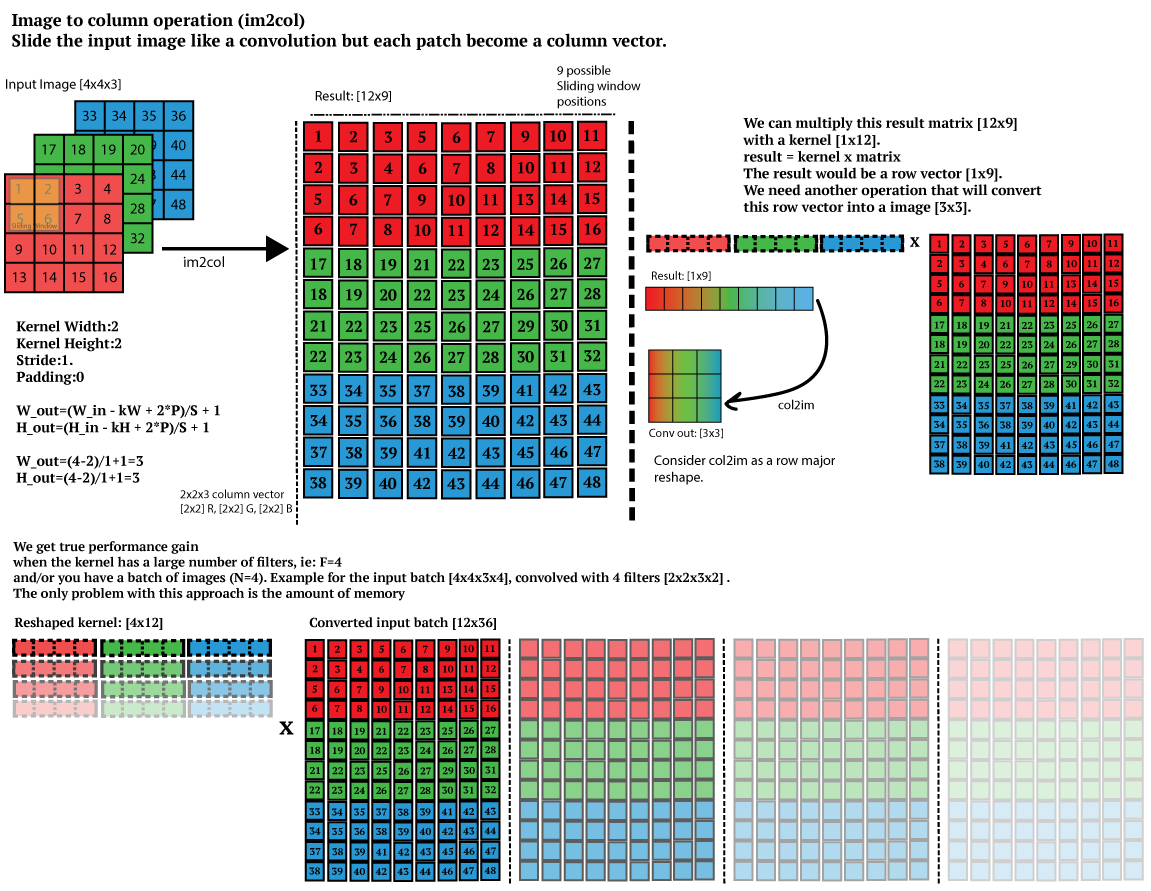
\includegraphics[width=15cm]{im2col.png}
    \caption{\textsf{im2col} algorithm scheme using a $2\times2$ filter on a image with 3 channels.
At the end of the \textsf{im2col} algorithm the \textsf{GEMM} is performed between weights and input image.
}
    \label{fig: convolutional layer _2}
\end{figure}

Another important optimization comes from linear algebra considerations and is called "Coppersmith-Winograd" algorithm, which was designed to optimize the matrix product. 
Suppose we have an input image of just 4 elements and a 1-D filter mask with size 3:
\begin{equation}
    \label{img_matrix}
img = \begin{bmatrix} 
	d0 & d1 & d2 & d3
	\end{bmatrix}
 \hspace{1cm}
weights = \begin{bmatrix} 
	g0 & g1 & g2
	\end{bmatrix}
\end{equation}
we can now use the im2col algorithm previously described and reshape our input image
and weights into
immagine
\begin{equation}
    \label{img_matrix_reshape}
img = \begin{bmatrix} 
	d0 & d1 & d2 \\
        d1 & d2 & d3 \\
 
	\end{bmatrix}
 \hspace* {1cm} ,  \hspace* {1cm}
weights = \begin{bmatrix} 
	g0 \\ 
        g1 \\ 
        g2
	\end{bmatrix}
\end{equation}
given this data, we can simply compute the output as the matrix product of this two
matrices:
\begin{equation}
    \label{output_matrix}
output = \begin{bmatrix} 
	d0 & d1 & d2 \\
        d1 & d2 & d3 
 
	\end{bmatrix}
 \hspace* {1cm}
    \begin{bmatrix} 
	g0 \\ 
        g1 \\ 
        g2
	\end{bmatrix}
\hspace* {1cm}
 = \begin{bmatrix} 
	d0\cdot g0 + d1 \cdot g1 + d2 \cdot g2 \\
        d1\cdot g0 + d2 \cdot g1 + d3 \cdot g2 \\
        \end{bmatrix}
        \end{equation}



The Winograd algorithm rewrites this computation as follow:
\begin{equation}
    \label{out_winograd}
output = \begin{bmatrix} 
	d0 & d1 & d2 \\
        d1 & d2 & d3 \\
 
	\end{bmatrix}
 \hspace* {1cm}
 \begin{bmatrix} 
	g0 \\ 
        g1 \\ 
        g2
	\end{bmatrix}
\hspace* {1cm}
= \begin{bmatrix}
        m1 + m2 +m3\\
        m2 -m3 -m4
        \end{bmatrix}\end{equation}
where
\begin{align*}
    \label{m1_4}
    m1 = (d0-d2)g0\hspace* {1cm}  m2 = (d1+d2)\frac{g0+g1+g2}{2} \\
    m4 = (d1-d3)g2\hspace* {1cm}  m3 = (d2-d1)\frac{g0-g1+g2}{2}
\end{align*}

The two fractions in m2 and m3 involve only weight's values, so they can be computed once per filter. Moreover, the normal matrix multiplication is composed of 6 multiplications and 4 addition, while the Winograd algorithm reduce the number of multiplication to 4, that is very significant, considering that a single multiplication takes 7 clock-cycles and an addition only 3.
\\
backward propagaiton.


\subsubsection{Pooling}
Pooling operations are down-sampling operations. They reduce spatial dimensions of the input image.
These operations and CL are very similar. A kernel of dimension slides across the image of dimension.
Differently from CL, pooling operation parameters are previously set and can’t change during the training phase.
Pooling computes a new output including summary statistic of the output of the precedent layer.
Max pooling is one of the most diffuse pooling functions. It reports the maximum output within a rectangular neighborhood.as shown in fig \ref{fig:pooling}
Other examples of pooling function are the average, the L2 norm or a weighted average based on the distance from the central pixel.
Pooling is useful to make representation approximately invariant to small transition of the input.
Invariance to translation means that if we translate the input by a small amount, the values of most of the pooled outputs do not change.
Invariance to local translation can be a useful property if we care more about whether some feature is present than exactly where it is.
Because pooling summarizes the responses over a whole neighborhood, it is
possible to use fewer pooling units than detector units, by reporting summary
statistics for pooling regions spaced k pixels apart rather than 1 pixel apart.
\\
The reductions of features can also prevent over-fitting problems during training, improving the general performances of the model.
A pooling layer is defined by the same parameters as a CL, minus the number of filters. 
Moreover, also the output dimensions for Pooling layers are the same as for CLs,however, they have no weights to be trained.
An example of pooling in fig \ref{fig:pooling}
\begin{figure}[htp]
    \centering
    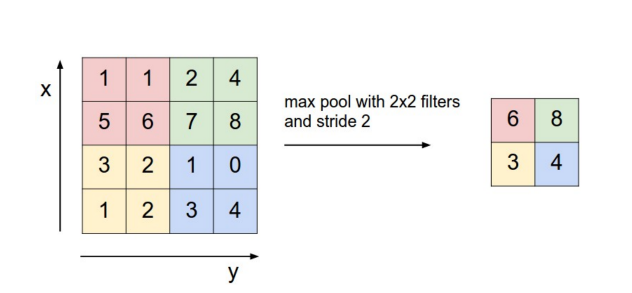
\includegraphics[width=15cm]{pooling.png}
    \caption{fig:pooling}
    \label{fig:pooling}
\end{figure}

    retroprop errore

\subsubsection{Shortcut Connections}

Shortcut connection represent an important improvement in in network architecture. It is well know that deep models suffer from degradation problem after reaching  a maximum depth. The construction of deep neural network brought some problems. The degradation problem is one of them and come out after reaching a maximum of depth. Adding a lot of layers saturate the model accuracy. This can decrease very rapidly proceeding in deeper layers.
This phenomena is caused by  error backward propagation. The error is multiplied lots of time and this can cause an explosion or vice versa a strong reduction of the error. This problem is well known in Deep Learning and takes the name of vanishing/exploding gradients.
This problem make very difficult the training of large model because deeper layers can’t easily learn even after lots of epoch.
A residual connection is a special shortcut which connects 2 different part of the network with a simple linear combination. Instead of learning a function  $ F(x)$  we try to learn  
$H(x) = F(x) + x$, as shown in figure \ref{fig:shortcut}:
During the back propagation the gradient of higher layers can easily pass to the lower layers, without being mediated, which may cause vanishing or exploding gradient.
\begin{figure}[htp]
    \centering
    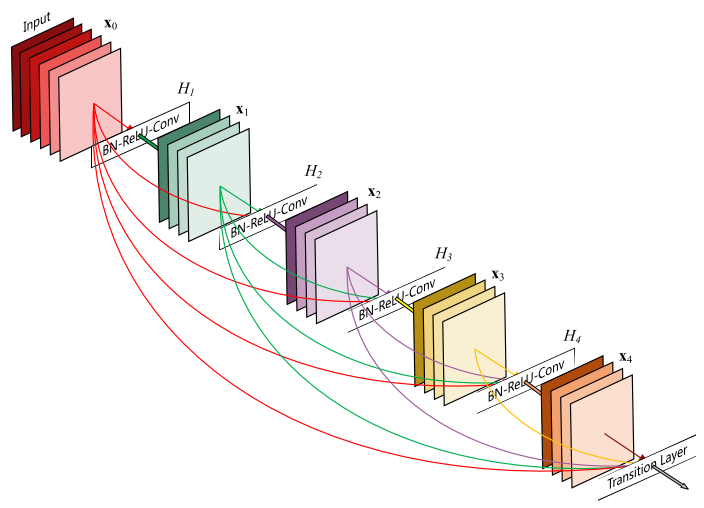
\includegraphics[width=10cm]{shortcut_layer.png}
    \caption{Scheme of shortcut connections into a deep learning model.
Each colored line connects the previous layer block to the following one.
The output combination can be customized but the most used one is a simple linear combination of them.
A particular attention must be paid with the dimensions management.
}
    \label{fig:shortcut}
\end{figure}
retropagazione dell'errroe.
\\
\\
\\

\subsubsection{Pixel Shuffle}
Using convolutional layers and pooling we have down-sampled the image and obtained an output, a feature maps, 
that hold the relevant feature of the input. In some application we are  interested in up-sampling the input, for example:
\begin{enumerate}
\item	In image to image processing
\item	Project feature maps to higher dimensional space. i.d to obtain a image of higher resolution (super resolution).
\end{enumerate}
For this purpose, the transpose convolution(deconvolution) was  introduced.
The transpose convolution can be seen as normal convolution with a sub-unitarian stride.
It work by up-sampling the input with empty columns and rows and then apply a  single stride convolution, as shown in figure \ref{fig:pixel_shuffle}
\begin{figure}[htp]
    \centering
    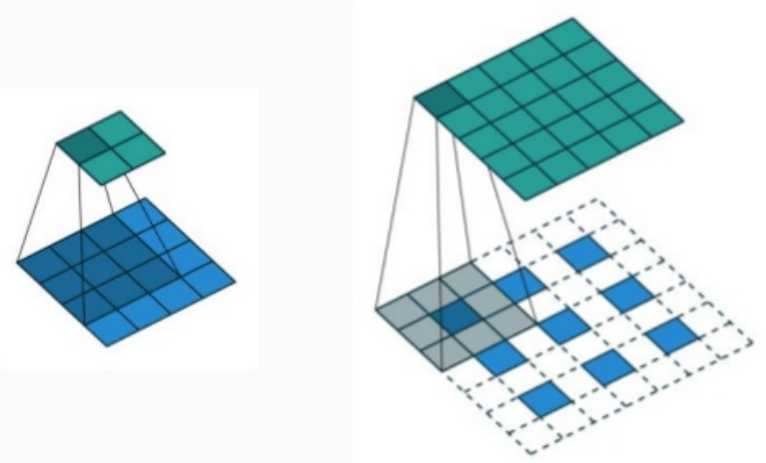
\includegraphics[width=10cm]{deconv.png}
    \caption{\href{text}{https://towardsdatascience.com/a-comprehensive-guide-to-convolutional-neural-networks-the-eli5-way-3bd2b1164a53 }}
    \label{fig:pixel_shuffle}
\end{figure}
This kind of process works but it is not computational and storage efficient.
To overcame these inefficiencies was recently introduced the sub-pixel convolution[].
This operation is just a rearrangements  of the pixel, it is totally deterministic and don’t require weights to be trained. 
Given a scale factor r, the PS organizes an input $H \times W \times C \times r2$ into an output tensor $ r \times H \times W \times C$ , which generally is the dimension of the high resolution space.
So, strictly speaking, the PS does not perform any up-sample, since the number of pixels stays the same. In figure \ref{fig:pixel_shuffle_sr} is shown an example with $ C = 1$:



 \begin{figure}[H]
        \centering
        \includesvg[width=0.5\textwidth]{pixel_shuffle.svg}
        \caption{Pixel Shuffle transformation.
On the left the input image with $scale^2$ (:= 9) channels.
On the right the result of Pixel Shuffle transformation.
Since the number of channels is perfect square the output is a single channel image with the rearrangement of the original ones.
}
\label{fig:pixel_shuffle_sr}
\end{figure}

    
As suggested by the authors[], the best practice to improve performances is to upscale from low resolution to high resolution only at the very end of the model. In this way the CL can efficiently produce an high number of low resolution feature maps that the PS can organize into the final output.
The backward function of this layer does not involve any gradient computation: instead, it is the inverse of the re-arrangement performed in the forward function.

\subsubsection{Batch Normalization}

The standard approach to train a neural network is to split the dataset in two groups, called batches or mini- batches. In this way the network can be trained with  multiple input at a time and the weights are updated by averaging in the batch.
We can define the batch size as the number of examples in each batch, that can vary from 1 to the number of example.
If the batch size is different from 1, there are some benefit. First the gradient loss over a mini-batch  is better estimate  of the gradient over the train set.
Second, due to parallel working of modern architecture it can be lot more efficient. 
Batch normalization is the operation that normalizes the features of the input along the batch axis, which allows to overcome a phenomenon in Deep Network training called internal covariate shift: whenever the parameters of the model change, the input distributions of every layer change accordingly.
This phenomena produce a slow down in the training convergence because each layer has to adapt itself to a new distribution of data for each epoch.
By making the normalization  a part of the model, the layer act also as a regularizer,  which allows better generalization performance.
Let's M be the number of examples in the group and $\epsilon $ a small variable added for numerical stability, the batch normalization function is defined as:
\begin{equation}
    \label{mu}
\mu = \frac{1}{M}\sum\limits_{i=1}^M x_i\end{equation}
\begin{equation}
    \label{theta}
\theta ^2 = \frac{1}{M}\sum\limits_{i=1}^M (x_i -\mu)^2 \end{equation}
\begin{equation}
    \label{x_i}
\hat{x_i} = \frac{(x_i-\mu)^2}{\sqrt{\theta^2 + \epsilon}} \end{equation}
\begin{equation}
    \label{y_i}
y_i=\gamma\Bar{x_i}+\beta \end{equation}
where $\gamma$ and $\beta $ are the trainable weights of this layer. In the case of a tensor of images of size M $\times$ H $\times$ W $\times$ C all the quantities are multidimensional tensors as well and all the operations are performed element-wise.

\subsubsection{Activation Functions}
The choice of activation function is a topic of particular interest. They can be linear or non -linear, in this case the network can compute a wider range of function and learn more complex relations in data patterns. Functions process the neuron output and bound it to a defined range.
There are many activation functions. They were proposed during the year. It is difficult to find what is the best one, we can say that each one has its pro and cos in some situation and the user has to find itself the most suitable.
In table 2.1 is reported a full record of the activation functions and their derivatives implemented in Byron and NumPyNet. 
An important feature of any activation function, in fact, is that it should be differentiable
since the main procedure of model optimization implies the back-propagation of the error
gradients.
An important optimisation is to compute activation derivative function as a function of it. In this way there is a reduction In terms o number of operation and it alloes to apply the backward gradient directly on the output, without storing the un-activated one.
The most used activation function is the ReLu activation (rectified Linear Unit). This function guarantee sparsity ( representation of data more efficient than a dense one), a reduction of the vanish of the gradient and an easy and fast computation of both forward and backward.

\begin{table*}[h]
\centering
\begin{adjustbox}{max width=\textwidth}
\begin{tabular}{lcc}
\hline \rowcolor{darkgrayrow}
\textbf{Name} & \textbf{Equation} & \textbf{Derivative} \\
\hline

Linear   &  $f(x) = x$                              &  $f'(x) = 1$ \\

Logistic &  $f(x) = \frac{1}{1 + \exp(-x)}$         &  $f'(x) = (1 - f(x)) * f(x)$ \\

Loggy    &  $f(x) = \frac{2}{1 + \exp(-x)} - 1$     &  $f'(x) = 2 * (1 - \frac{f(x) + 1}{2}) * \frac{f(x) + 1}{2} $ \\

Relu     &  $f(x) = \max(0, x)$                     &  $f'(x) = \left\{\begin{array}{rlr}
                                                                       1   & \mbox{if} & f(x) > 0    \\
                                                                       0   & \mbox{if} & f(x) \leq 0
                                                                       \end{array}\right.$           \\

Elu      &  $f(x) = \max(\exp(x) - 1, x)$           &  $f'(x) = \left\{\begin{array}{rlr}
                                                                       1        & \mbox{if} & f(x) \geq 0 \\
                                                                       f(x) + 1 & \mbox{if} & f(x) < 0
                                                                       \end{array}\right.$                \\

Relie    &  $f(x) = \max(x * 1e-2, x) $             &  $f'(x) = \left\{\begin{array}{rlr}
                                                                       1    & \mbox{if} & f(x) > 0    \\
                                                                       1e-2 & \mbox{if} & f(x) \leq 0
                                                                       \end{array}\right.$            \\

Ramp     &  $f(x) = \left\{\begin{array}{rlr}
                            x^2 + 0.1 * x^2 &  \mbox{if} & x > 0    \\
                            0               &  \mbox{if} & x \leq 0
                           \end{array}\right.$
                                                    &  $f'(x) = \left\{\begin{array}{rlr}
                                                                       f(x) + 1 & \mbox{if} & f(x) > 0   \\
                                                                       f(x)     & \mbox{if} & f(x) \leq 0
                                                                       \end{array}\right.$               \\

Tanh     &  $f(x) = \tanh(x)$                       &  $f'(x) = 1 - f(x)^2$  \\

Plse     &  $f(x) = \left\{\begin{array}{rlr}
                            (x + 4) * 1e-2     & \mbox{if} & x < -4           \\
                            (x - 4) * 1e-2 + 1 & \mbox{if} & x > 4            \\
                            x * 0.125 + 5      & \mbox{if} & -4 \leq x \leq 4
                           \end{array}\right.$
                                                    &  $f'(x) = \left\{\begin{array}{rlr}
                                                                       1e-2  & \mbox{if } & f(x) < 0 \mbox{ or } f(x) > 1 \\
                                                                       0.125 & \mbox{if } & 0 \leq f(x) \leq 1
                                                                       \end{array}\right.$                                \\

Leaky    &  $f(x) = \left\{\begin{array}{rlr}
                            x * C &  \mbox{if} & x \leq 0 \\
                            x     &  \mbox{if} & x > 0
                           \end{array}\right.$
                                                    &  $f'(x) = \left\{\begin{array}{rlr}
                                                                       1   & \mbox{if} & f(x) > 0    \\
                                                                       C   & \mbox{if} & f(x) \leq 0
                                                                       \end{array}\right.$           \\

HardTan  &  $f(x) = \left\{\begin{array}{rlr}
                            -1 & \mbox{if} &     x < -1 \\
                            +1 & \mbox{if} &     x > 1  \\
                             x & \mbox{if} & -1 \leq x \leq 1
                           \end{array}\right.$
                                                    &  $f'(x) = \left\{\begin{array}{rlr}
                                                                        0 & \mbox{if} & f(x) < -1 \mbox{ or } f(x) > 1 \\
                                                                        1 & \mbox{if} & -1 \leq f(x) \leq 1
                                                                       \end{array}\right.$                            \\

LhTan    &  $f(x) = \left\{\begin{array}{rlr}
                            x * 1e-3           & \mbox{if} &     x < 0  \\
                            (x - 1) * 1e-3 + 1 & \mbox{if} &     x > 1  \\
                             x                 & \mbox{if} & 0 \leq x \leq 1
                           \end{array}\right.$
                                                    &  $f'(x) = \left\{\begin{array}{rlr}
                                                                        1e-3           & \mbox{if} & f(x) < 0 \mbox{ or } f(x) > 1 \\
                                                                        1              & \mbox{if} & 0 \leq f(x) \leq 1
                                                                       \end{array}\right.$                                  \\

Selu     &  $f(x) =\left\{\begin{array}{rlr}
                            1.0507 * 1.6732 * (e^x - 1) & \mbox{if} &    x < 0  \\
                            x * 1.0507                  & \mbox{if} &    x \geq 0
                           \end{array}\right.$

                                                    &  $f'(x) = \left\{\begin{array}{rlr}
                                                                        f(x) * 1e-3           & \mbox{if} & f(x) 0    \\
                                                                        (f(x) - 1) * 1e-3 + 1 & \mbox{if} & f(x) > 1  \\
                                                                        \end{array}\right.$                           \\

SoftPlus &  $f(x) = log(1 + e^{x})$                 &  $f'(x) = \frac{\exp(f(x)}){1 + e^{f(x)}}$ \\

SoftSign &  $f(x) = \frac{x}{|x| + 1}$              &  $f'(x) = \frac{1}{(|f(x)| + 1)^{2}}$ \\

Elliot   &  $f(x) = \frac{\frac{1}{2} * S * x}{1 + |x + S|} + \frac{1}{2}$

                                                    &  $f'(x) = \frac{\frac{1}{2} * S}{(1 + |f(x) + S|)^{2}} $ \\

SymmElliot &  $f(x) = \frac{S * x}{1 + |x * S|}$    &  $f'(x) = \frac{S}{(1 + |f(x) * S|)^{2}}$ \\


%Swish    &  $f(x) = $                               &  $f'(x) = $                                                                                            %\\

%SoftMax  &  $f(x) =\frac{\exp(x)}{\sum_{i=1}^{N}x}$ &  $f'(x) = $


\hline\\
\end{tabular}
\end{adjustbox}
\caption{List of common activation functions with their corresponding mathematical equation and derivative.
The derivative is expressed as function of $f(x)$ to optimize their numerical evaluation.}
\end{table*}

\subsection{Cost Function}

At the Base of deep learning training there is the minimization of a Cost function. During the training we adjust the parameters of the network in order modify the output and make it closer to desire one.
Therefore, it is important to choose the most appropriate error function. An important property of a loss function is its differentiability, since it is the starting point if the chain rule for derivatives used in Error Backpropagation.
The most common cost functions for Super Resolution are Mean squared Error
the fomrer is defined as:

$$ MSE = \frac{1}{N}\sum\limits_{i=1}^N (y_i - t_i)^2$$
where y is the output vector of de model, t is the desired results and N is the output dimension. It is very simple and reaches good perfomances.

the MAE is defined as:
$$ MAE = \frac{1}{N}\sum\limits_{i=1}^N \left|(y_i - t_i) \right|$$

\chapter{DATASET AND METHODOLOGY} 
Image super resolution  problem has gained research attention for decades.
The goal of super resolution is to obtain an high resolution image from a low resolution one.
Many studies assume that a low resolution image is a bicubic downsample of an high resolution image.But other factor like noise degrading can be considered.
Recently SR models have shown improvement in terms of PSNR. Howevere such models exhibit limitation in terms of architecture optimality.
Their reconstruction performance is sensitive to minor architectural changes. These models reach different levels of performance by different initialitaion and training techniques.
Thus, designed model architecture and  sophisticated optimization methods are essential in training the neural network.

In the next section will be introduced EDSR model,that is the state of art Deep Neural Network specialized in Single Image Super Resolution (SISR) which won the NTIRE challenge in 2017.

\section{EDSR}
Edsr can be considered an upgrade of SSResNet,a ResNet type network, that have been already  applied successfully to super resolution. However we consider EDSR a further improvement of SSResNEt, employing better ResNet structures. 
The base unit of {\tt EDSR} is the {\it residual block}, which makes extensive use of {\it residual connections}, described in the previous chapter.
\\
The author improved the model by removing the batch normalization layers, since they get rid of range flexibility from networks by normalizing the features. As shown in fig \ref{convnet}
\begin{figure}[H]
    \centering
    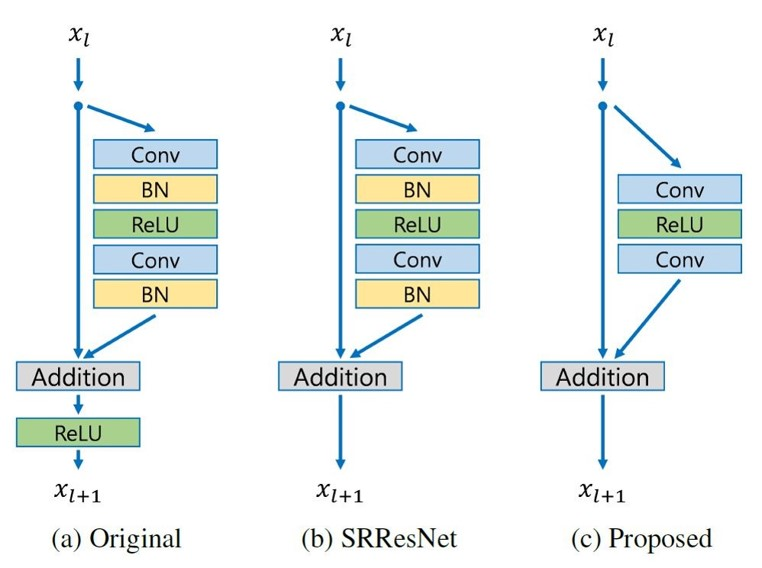
\includegraphics[scale=0.8]{ConvNEt.jpg}
    \caption{Comparison of residual blocks in original
ResNet, SRResNet, and EDSR.}
    \label{convnet}
\end{figure}
Furthermore, memory usage is reduced by 40\% since batch normalization layers consume the same amount of memory as preceding convolutional layers.
Consequently it si possible to build up a largere model that  has better performance thanconventional ResNet structure under limited computational
resources.
Furthermore, the authors solved the problem of deepening the models by e by adopting a residual scaling in shortcut connection with factor 0.1. In each residual block, constant scaling layers are placed after the last convolution layers. 
 \\
The structure of the model is summarize in figure \ref{fig:edsr-structure}:
A fisrt Convolutional layers, using 256 filters, processes the input LR image. Than a set of 32 residual blocks process the feature map, each residual block in turn composed by:
\begin{itemize}
 \setlength\itemsep{-0.3em}
 \item a convolutional layer with 256 filters
 \item an activation layer with a ReLU function
 \item a convolutional Layer with 256 filters
 \item a linear combination (pixel-by-pixel) with the input of the residual block with weight respectively 0.1 and 1
\end{itemize}

 The last part of the architecture is composed by an up-sample block which re-organize the pixels using a series of convolution layers w and pixel-shuffle functions. The up-sampling follows the scale factor imposed: the model increases the spatial resolution of the image by a fixed scale factor (x2  in our applications) and each pixel-shuffle application is equivalent to a x2 in the output sizes 1.
 The tail of the network is composed by a shortcut connection between the initial input with the output of the 32 residual block and by the up-sampling block:
 
\begin{itemize}
 \setlength\itemsep{-0.2em}
 \item A convolutional layer with 1024 filters 
 \item A pixel-shuffle
 \item A convolutional layer with 3 filter that retunr the final output
\end{itemize}
The model increases the spatial resolution(pixel-shuffle) of the image by a fixed scale factor x2 

\begin{figure}[H]
 \centering
 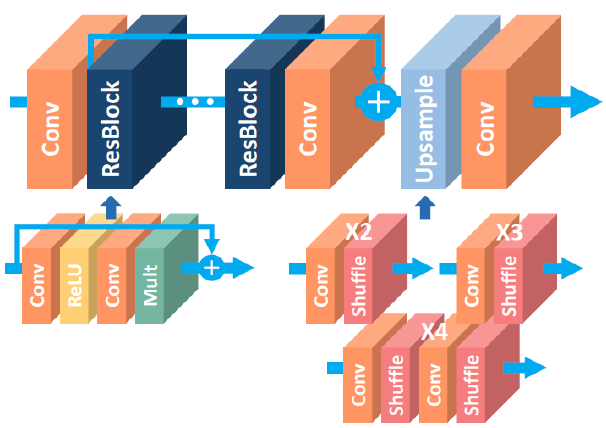
\includegraphics[scale=0.4]{edsr_structure.png}
 \caption{\it architecture of the single scale SR Network (EDSR)}
 \label{fig:edsr-structure}
\end{figure}




  EDSR has a totally  more than 40 millions of parameters, summarized in table \ref{tab:edsr-weights}



\begin{table}[H]
\begin{center}
\setlength{\tabcolsep}{14pt}
\begin{tabular}{|l l l l|}
 \hline
 Layer & Channels in/out & Filters Dim. & Parameters \\
 \hline
 Conv. Input       & 3 / 256     & 3x3 & 6912\\ [0.3cm]
 Conv. Res. Block        & 256 / 256   & 3x3 & 1179648\\[0.3cm]
 Conv. Pre Short.  & 256 / 256   & 3x3 & 589824\\[0.3cm]
 Conv. Pre-Shuffle & 256 / 1024  & 3x3 & 2359296 \\[0.3cm]
 Conv. Output      & 256 / 3     & 3x3 & 6912\\
 \hline
\end{tabular}
\end{center}
\caption{\it Table of parameters for the different sections of EDSR.}
\label{tab:edsr-weights}
\end{table}

The Residual Blocks section, with more than 37 millions of parameters is the "heaviest" part of the model.
\\
For training they used $48 \times 48$ RGB patches from LR images (from DIV2K) with the corresponding HR patches, augmenting the training data with random horizontal flips and 90° rotations. 
The optimizer is the ADAM  and the loss function is the L1: even if the L2 naturally maximize the PSNR (which is the only metrics evaluated in the challenge), they found that L1 loss provided a better convergence.
\\
For training they used $48 \times 48$ RGB input patches of size
from LR image with the corresponding HR patches from DIV2K.
they augmented the training data with random horizontal flips
and 90° rotations. 
The optimizer is the ADAM.
the authors trained the networks using L1 loss instead of L2. Minimizing L2 generally maximizes the PSNR. However, they empirically found that L1 loss provides better convergence
than L2. 



\section{Training Dataset: DIV2K}

DIV2K dataset [26] is a newly proposed high-quality
(2K resolution) image dataset for image restoration tasks.
The DIV2K dataset consists of 800 training images, 100
validation images, and 100 test images. As the test dataset
ground truth is not released, we report and compare the performances on the validation dataset. We also compare the
performance on four standard benchmark datasets: Set5 [2],
Set14 [33], B100 [17], and Urban100 [10].


The training dataset employed for EDSR is called DIV2K and consist 1000 RGB images in dived into :
\begin{itemize}
 \setlength\itemsep{-0.8em}
\item 800 training immmages
\item 100 test images
\item100 validation images
\end{itemize}
Some qualitative results that can be obtained from EDSR compared with other model like Bicubic and WDSR,(i.e Wide Deep Super Resolution,the winner of the NTIRE challenge 2018, composed by 32 residual blocks, similar to EDSR, but much lighters, are shown in pictures \ref{fig:sky}, \ref{fig:city} and \ref{fig:windows}.
\begin{figure}[H]
  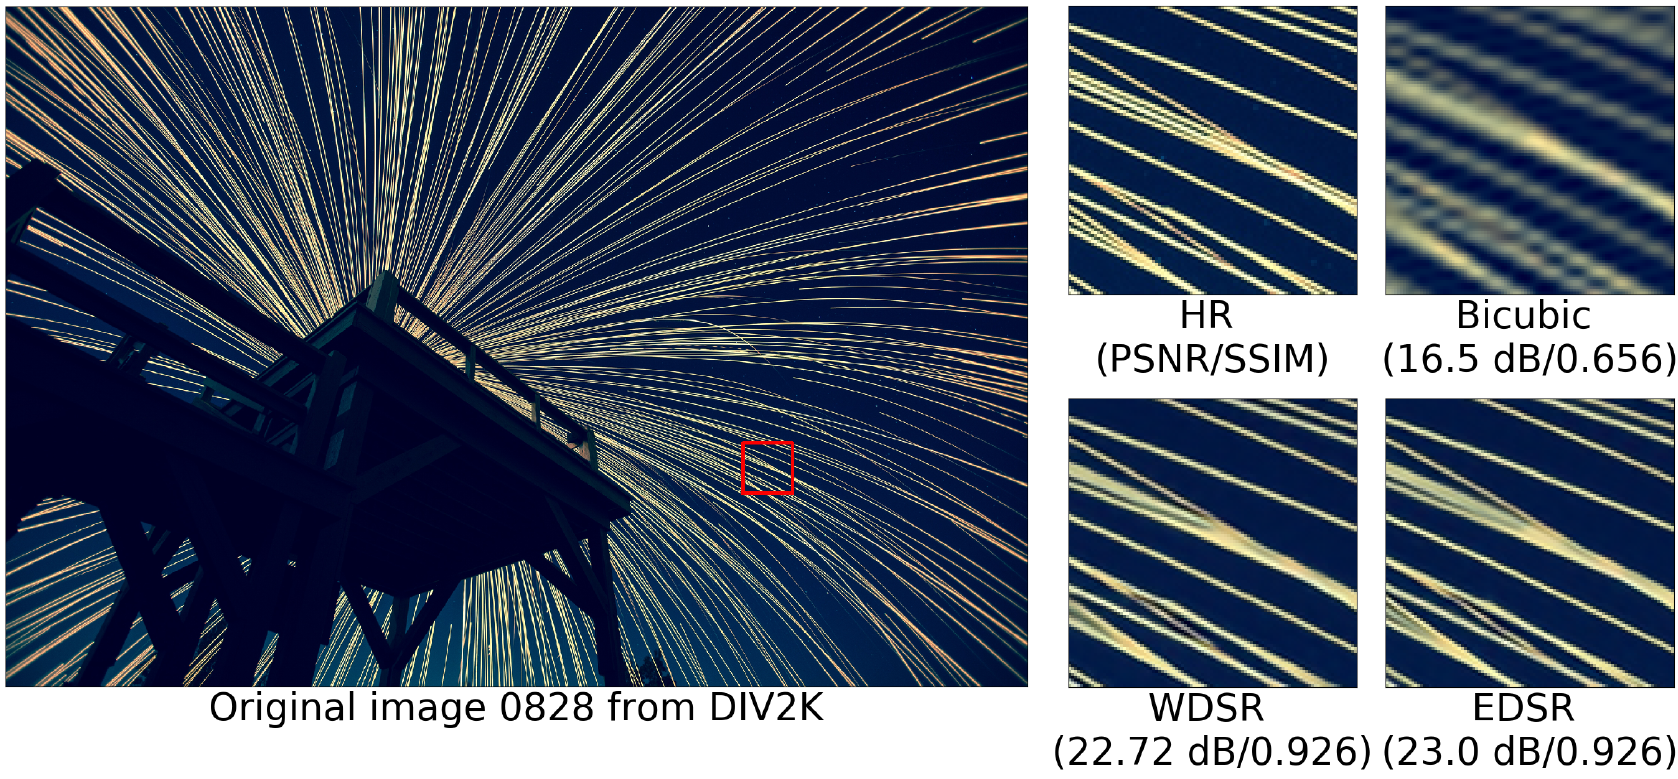
\includegraphics[scale=0.5]{sr_res1.png}
    \caption{\it Super Resolution visual example extracted from the DIV2K validation set. The quality score in terms of PSNR and SSIM are compared between a standard bi-cubic up-sampling and the EDSR and WDSR models.}
  \label{fig:sky}
\end{figure}

\begin{figure}[H]
  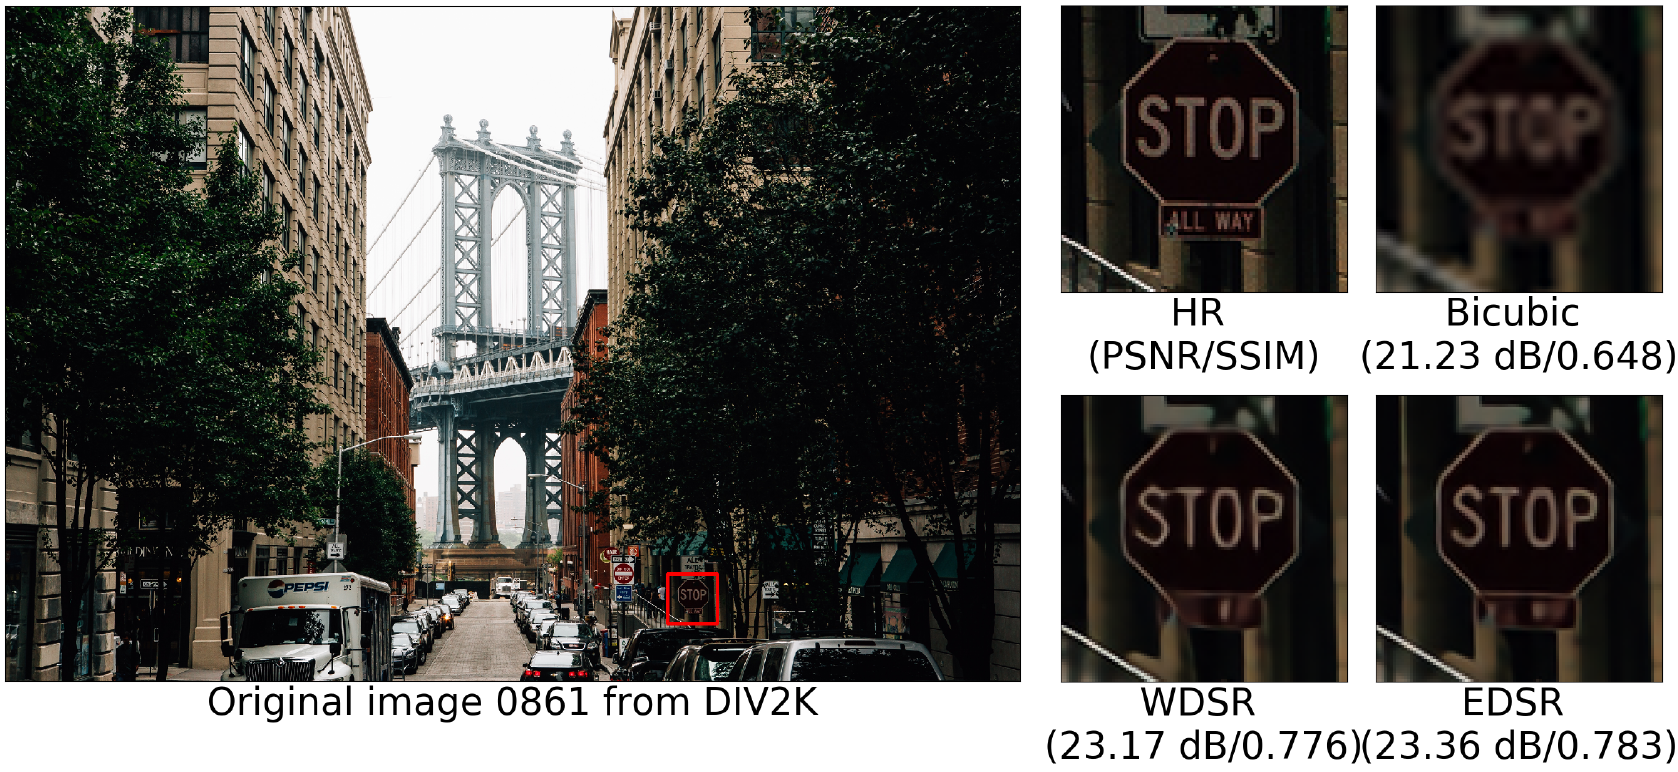
\includegraphics[scale=0.5]{sr_res2.png}
    \caption{\it Super Resolution visual example extracted from the DIV2K validation set. The quality score in terms of PSNR and SSIM are compared between a standard bi-cubic up-sampling and the EDSR and WDSR models.}
  \label{fig:city}
\end{figure}

\begin{figure}[H]
  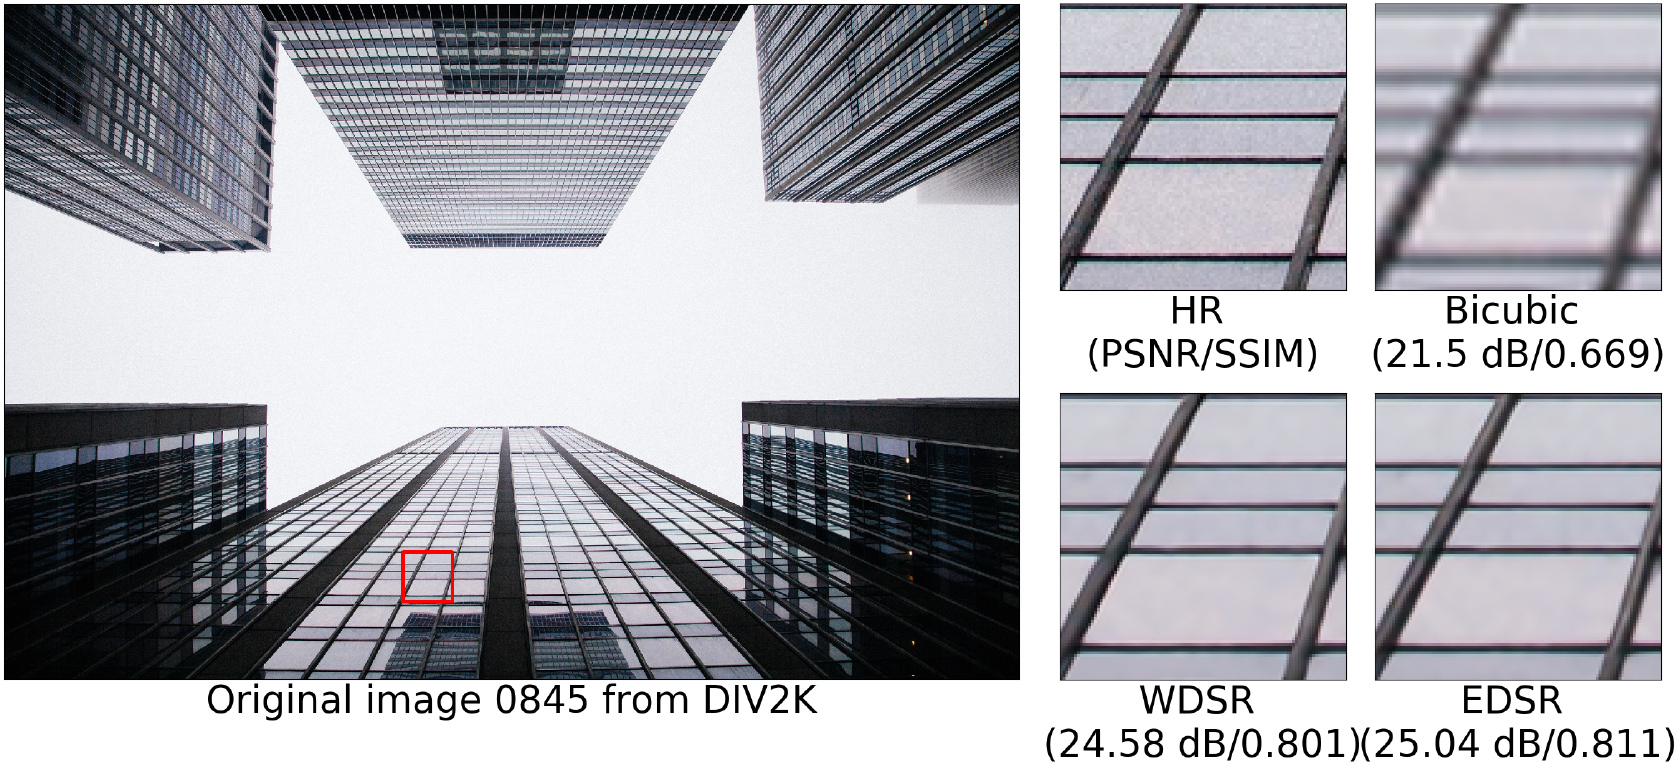
\includegraphics[scale=0.5]{sr_res3.png}
  \caption{\it Super Resolution visual example extracted from the DIV2K validation set. The quality score in terms of PSNR and SSIM are compared between a standard bi-cubic up-sampling and the EDSR and WDSR models.}
  \label{fig:windows}
\end{figure}
The results show that the EDSR model have learned how to interpolate different kind of texture and complex line shape better than Bicubic algorithm and WDSR model
\\
The model was trained on a huge heterogeneous set of data. The model during the training phase saw a lot of different texture, therefore it is able  to reconstruct a huge amount of distinct shapes and textures. For this reasons we decided to test the performances of   EDSR on 
 different set of data like  Mnsit database, some histopathology in fluorescence and MR images without a model re-training.



\section{Mnist DataSet}
The MNIST database (Modified National Institute of Standards and Technology database) is a large database of handwritten digits that is commonly used for training various image processing systems.The database is also widely used for training and testing in the field of machine learning.It was created by "re-mixing" the samples from NIST's original datasets.The black and white images from NIST were normalized to fit into a 28x28 pixel bounding box and anti-aliased, which introduced grayscale levels.
The MNIST database contains 60,000 training images and 10,000 testing images.
\begin{figure}[H]
    \centering
    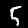
\includegraphics[scale=1]{mnist.png}
    \caption{mnist}
    \label{fig:mnist}
\end{figure}

EDSR  has been applied on images with diffeent features. 
\section{Histopathology Fluorescence DataSet}
Fluorescence microscopy is a type of an optical microscopy that uses fluorescence to image 3D subcellular
structures .
Fluorescence imaging relies on illumination of fluorescently labeled proteins or other intracellular molecules with a defined wavelength of light ideally near the peak of the fluorophor excitation spectrum, and detection of light emitted at a longer wavelength.
The images used in this work are taken from
S-BSST265 FLUORESCENCE DATASET.
I applied SR on these images with the aim of analyze how EDSR work on images with  different type of features, like contrast, color and texture.
To make fluorescence images compatible with EDSR algorithm, they were transformed in gray-scale images and then in RGB images.
\begin{figure}[H]
    \centering
    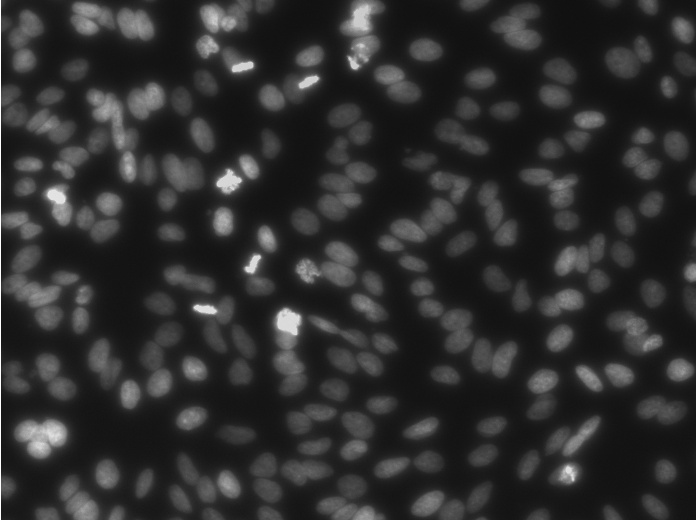
\includegraphics[scale=0.5]{c304a1fdf3bca2f4b4580d2cac59942e2224a7678001bf5ed9d9852f57708932.jpeg}
    \caption{Fluorescence image}
    \label{fig:Fluorescence}
\end{figure}
Other Deep learning field are applied on Fluorescence imaging. For example Segmentation Neural Network try  to quantify and characterize cells, nuclei or other biological
structures in these kind of images.
Applying SR on images before using segmentation improves spatial resolution and can improve separation between different structures in the images. Therefore, segmentation can be applied on higher quality images and detect more object.

\section {Bright field images}
Bright-field microscopy (BF) is the simplest of all the optical microscopy illumination techniques. Sample illumination is transmitted (i.e., illuminated from below and observed from above) white light, and contrast in the sample is caused by attenuation of the transmitted light in dense areas of the sample. Bright-field microscopy is the simplest of a range of techniques used for illumination of samples in light microscopes, and its simplicity makes it a popular technique. The typical appearance of a bright-field microscopy image is a dark sample on a bright background, hence the name.
\begin{figure}[H]
    \centering
    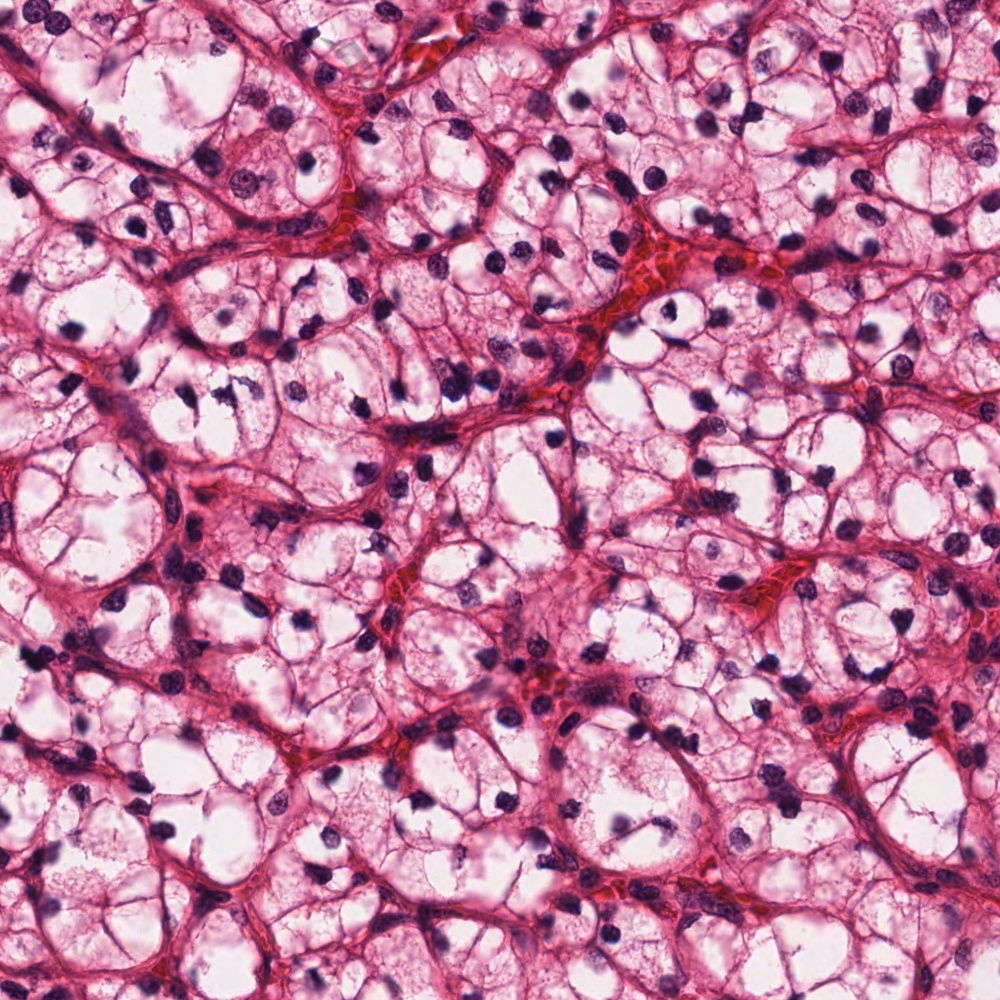
\includegraphics[scale=0.25]{TCGA-B0-5698-01Z-00-DX1.jpeg}
    \caption{fluo}
    \label{fluo_1}
\end{figure}
As the above datasets, this dataset was used in order to examine the versatility of SR.

\section{NMR DataSet}
To test the model on NMR images, we used a series of mammography NMR.
The goal is to enhance these images in order to better detect breast micro-calcification.
\begin{figure}[H]
    \centering
    \includegraphics{}
    \caption{breast NMR}
    \label{breast NMR}
\end{figure}

\chapter{Results}



\newpage
\thispagestyle{empty}
\listoffigures

\newpage
\nocite{*}
\bibliographystyle{abbrv}
\bibliography{sample}

\end{document}
